\documentclass[proseminar,german,utf8]{zihpub}

\usepackage{setspace}
\usepackage{hyperref}
\usepackage{graphicx}
\usepackage{subfig}

% Abkuerzungen typografisch korrekt
\newcommand{\zB}[0]{{z.\,B. }}
\newcommand{\ZB}[0]{{Z.\,B. }}
\renewcommand{\dh}[0]{{d.\,h. }}
\newcommand{\Dh}[0]{{D.\,h. }}
\newcommand{\iA}[0]{{i.\,Allg. }}
\newcommand{\ua}[0]{{u.\,a. }}
\newcommand{\ca}[0]{{c.\,a. }}

\author{Paul Gottschaldt}
\title{Julia - High-Performance Programmiersprache für High-Performance Computing?}
\matno{4609055}
\betreuer{Martin Schroschk}
\bibfiles{references}

\begin{document}

\section {Einleitung}
1998 startete das Apache-Point-Observatorium~\cite{APOWiki} in New Mexico (USA) ihr Projekt Sloan Digital Sky Survey (SDSS)~\cite{SDSSWiki} \cite{SDSSIII}, welches Fotos von über 35~\% aller sichtbaren Objekte unseres Himmels anfertigte und in einer Datenbank zunächst sicherte. Seit diesem Jahr wurden bereits über 500~Millionen Sterne und Galaxien fotografiert und Licht eingefangen, welches bereits Milliarden von Jahren unterwegs war und die Forscher bis weit in die Vergangenheit unseres Universums zurückblicken lässt. Die SDSS-Kamera galt bis zu ihrer Abschaltung im Jahr 2009 als produktivste Weltraumkamera der Welt. Mit etwa 200~GB reine Bilddaten pro Nacht entstand so eine Datenbank mit über 5~Millionen Bildern von jeweils 12~Megabyte - zusammengerechnet also rund 55~Terabyte~\cite{CelesteV2}. 2014 startete ein Team von Astronomen, Physikern, Informatikern und Statistikern das Projekt Celeste, um eben jenen Datensatz zu katalogisieren und für jeden Himmelskörper einen Eintrag anzulegen~\cite{CelesteV3}. In der ersten veröffentlichten Version von 2015 noch auf Berechnungen auf einzelne Knoten beschränkt, schaffte es das Forschungsteam um die involvierten Parteien Julia Computing, UC Berkeley, Intel, National Energy Research Scientific Computing Center (NERSC) und Lawrence Berkeley National Laboratory in der zweiten Version von 2016 bereits einen 225-fachen Geschwindigkeitsgewinn zu erzielen. Die größten Verbesserungen waren dabei der mit 8192 Intel® Xeon® Prozessoren ausgestattete Hochleistungsrechner( zu engl. High-Performance-Computer oder HPC) des Berkeley Lab's und Julia, eine High-Performance Open-Source Programmiersprache, die bis dato noch relativ unbekannt war und seit 2009 am MIT entwickelt wird. ~\cite{CelesteHeise} \cite{CelesteVideo} Besonders ist an Julia vorallem ihr Anspruch, eine sehr produktive (high-programming language) wie Python zu sein, dabei aber Performanz wie C zu erreichen. Im November 2017 veröffentlichte dieses Team dann die aktuelle dritte Version, mit der sie nochmals einen deutlichen Geschwindigkeitsgewinn erreichen konnten. Sie schafften es 188 Millionen Sterne und Galaxien in nur 14,6 Minuten zu katalogisieren und nutzten dafür bis zu 1,3 Millionen Threads auf den 9300 Knights Landing(KNL) Knoten des Cori Supercomputers des NERSC. Dabei erzielten sie mit Julia eine Peak-Performance von 1,54 Petaflop pro Sekunde für Berechnungen mit doppelter Genauigkeit. Damit erzielte das Celeste Projekt einen 100-fachen Performanzgewinn zu allen vorherigen Forschungsprojekten. Derzeit gibt es rund 200 Supercomputer in der Welt, welche in der Lage sind eine Peak-Performance von mehr als einem Petaflop pro Sekunde zu erreichen. Trotzdem sind so gut wie alle Anwendungen, welche eben jene Peak-Performance erreichen von wenigen Gruppen von Experten geschrieben, welche ein sehr tiefes Verständnis für alle erforderlichen Details besitzen~\cite{CelesteNextPlatform}. Umso erstaunlicher ist an diesem Ergebnis also die Tatsache, dass das Team hinter Celeste die Geschwindigkeit ausschließlich unter Nutzung ihrer Kenntnisse, dem Julia-Code und dessen Threading-Model erzielen konnten.

\begin{figure}[hbt!]
  \centering
  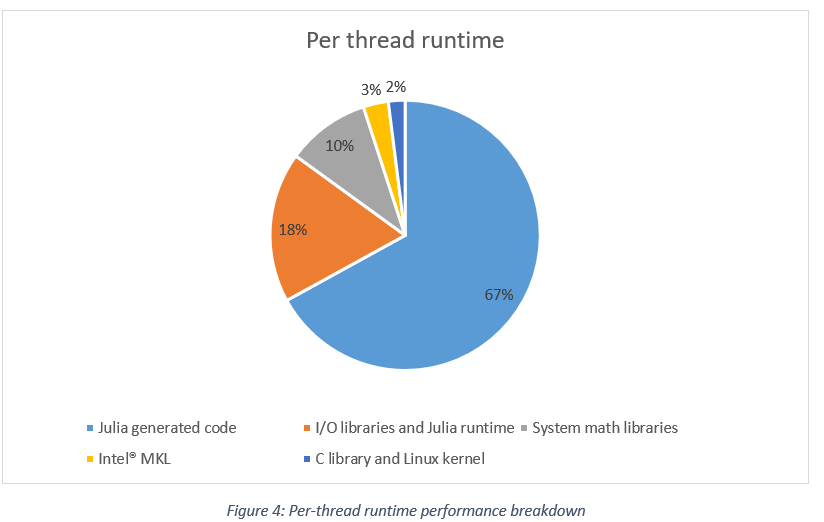
\includegraphics[scale=0.65, trim={5mm 10mm 5mm 5mm},clip]{bilder/celestejulia.png}
  \caption{Die pro Thread Auslastung des Celeste-Projekts}
  \cite{CelesteNextPlatform}
  \label{fig:celestejulia}
\end{figure}

In Abbildung~\ref{fig:celestejulia} ist die pro Thread Auslastung des Celeste-Projekts in Version 3 dargestellt. Zu sehen ist, dass Julia 82,3~\% der Zeit lief und damit auch diesen Anteil an der Performanz liefert. Damit stellt Julia unter Beweis das es sowohl für TheraByte-große Datensätze, wie auch für Petaflop pro Sekunde-schnelle Berechnungen geeignet ist. Keno Fischer, CTO von Julia Computing, sagte 2017, das Projekte wie Celeste unter Beweis stellen, das der Traum, der hinter Julia steht, wahr wird. Wissenschaftler können nun auf ihrem Rechner entwickelte Prototypen einfach von ihrem Laptop auf die größten Supercomputer verschieben ohne zwischen Sprachen wechseln zu müssen oder ihren Code gar komplett neu zu schreiben. Sie (Anmerkung: Entwickler von Julia Computing) sind sehr stolz darauf, dies alles geschafft zu haben und glauben sehr daran, das Julia die Entwcklung in der Forschung für viele Jahre sehr voranbringen wird. Viral Shah, CEO von Julia Computing, sagte das Forscher sich nun auf die Lösung ihrer Probleme fokussieren können und sich nicht mehr mit dem Programmieren beschäftigen müssen~\cite{CelesteV2}.
%%%%%%%%%%%%%%%%%%%%%%%%%%%%%%%%%%%%%%%%%%%%%%%%%%%%%%%%%%%%%%%%%%%%%%%

\section{Einführung in die Programmiersprache Julia}

\subsection{Übersicht}

Julia ist eine junge, flexible, höhere Programmiersprache, die es sich selbst als Ziel gesetzt hat, die hohe Produktivität und einfache Handhabbarkeit aus Sprachen wie Python mit der großen Geschwindigkeit von C zu kombinieren. Auch wenn sie vorallem für wissentschaftliches und numerisches Rechnen gestaltet worden ist, bietet sie eine sogleich performante wie auch einfach zu lernende Umgebung und versucht damit den derzeitigen Trend von mehrsprachigen Softwarelösungen in der Wissenschaft entgegen zu wirken. Mit einer Syntax die an eine Kombination aus MATLAB und Python erinnert, Lisp-ähnlichen Macros und Metaprogrammierung, einem Compiler der \textit{LLVM} nutzt und einem eigenem Paketmanager der an \textit{Git} angelehnt ist, hat sich Julia viele bereits etablierte Funktionen zunutze gemacht. Zusätzlich besitzt sie die Möglichkeit C- und Python-Funktionen einfach direkt aufzurufen, was die Nutzung der Bibliotheken der beiden Sprachen direkt im Julia-Code ermöglicht. Julias gute Performanz wird vorallem durch Multimethoden für einzelne Funktionen und die automatische Generierung von effizientem typspezialisierten Code gewonnen. Dabei ist Julia sowohl dynamisch als auch statisch typisiert. Zudem ist Julia funktional, objektorientiert und imperativ und wurde fast komplett in Julia selbst geschrieben. ~\cite{NominalTypSystemWiki}~\cite{TypSystemWiki}~\cite{JuliaLangIntro}~\cite{JuliaBasicHeise}
%%%%%%%%%%%%%%%%%%%%%%%%%%%%%%%%%%%%%%%%%%%%%%%%%%%%%%%%%%%%%%%%%%%%%%%

\subsection{Typensystem und Multimethoden}

In Julia gibt es keine Klassen, wie es sonst für objektorientierte Sprachen üblich ist. Stattdessen werden in Julia Daten eines Objektes explizit von dessen Methoden getrennt. Vom Nutzer angelegte Objekte, wie sie aus anderen puren objektorientierten Sprachen wie C++ oder Java bekannt sind, ähneln am meisten dem \textit{Composite Types}. Auch bekannt unter Namen wie \textit{struct} oder \textit{records} stellt er eine Ansammlung von benannten Feldern da. Diese einzelnen Felder können wie einzelne Attribute betrachtet werden und besitzen einen Wert. Im Sinne der Objektorientierung können die \textit{Composites} ineinander verschachtelt werden. Zusätzlich erzeugt Julia standartmäßig für jeden \textit{Composite Type} auch Konstruktoren. Auch wenn Julia dynamisch ist und damit der Typ eines Wertes nicht angegeben werden muss, besitzt jeder einen festen Datentyp. Dies gilt auch für die vom Nutzer erstellten Typen.  Datentypen existieren dabei nur zur Laufzeit und entsprechen genau dem aktuellen Typ, den ein Wert während der Ausführung besitzt. Auch besitzen nur Werte einen Typ, eine Variable stellt lediglich einen Namen gebunden an einen Datentyp dar. Julias Rückgrat für das Typensystem sind die abstrakten Datentypen. Während ein Wert immer einen konkreten Datentyp besitzt, ist dieser Typ gleichzeitig in einen Graphen von abstrakten Typen eingebunden. Konkrete Typen sind die Knoten dieses Graphen und können keine Elternknoten sein. Abstrakte Typen dagegen können mehrere Kinder- und Elternknoten besitzen und bilden die Basis von Julia. Der Datentyp \textit{Int64} ist \zB Kindknoten vom abstrakten Typ \textit{Signed}, welcher Kindknoten vom Typ \textit{Integer} ist. Als oberster Knoten steht der Datentyp \textit{Any}. Ein Nutzer kann seine definierten Objekte in diesen Graphen einfügen. Wird nichts weiter spezifiziert, wird das Objekt standartmäßig als Kind vom Typ \textit{Any} angenommen. Als ein weiteres Feature unterstützt Julia auch parameterisierte Datentypen. Diese ermöglichen die generische Erstellung von vielen kombinierten Datenypen und dienen zudem unterstützend für Julias weiteres Schlüsselmerkmal - die Multimethoden. Im Kontext von Julia stellen Funktionen ein Objekt dar, welches ein Tuple von Eingangswerten einem Rückgabewert zuordnet oder einen Fehler wirft. Eine einzelne Funktion fasst dabei einen Sachverhalt wie \zB die Addition von Werten zusammen und besitzt unterschiedlich viele verschiedene Methoden, welche je nach Anzahl der Argumente und Typ jedes einzelnen Wertes gewählt wird. Deshalb werden Funktionen in Julia auch generisch genannt. Methoden widerrum sind nun eine explizite Implementierung einer Funktion und werden nach dem Multimethoden-Verfahren (in Englisch multiple dispatch) ausgewählt. Damit grenzt sich Julia im Sinne des objektorientierten Paradigmas sehr von Sprachen wie Java oder C++ ab. Während in diesen Sprachen eine Zuordnung nach dem Typ des ersten Arguments (single dispatch) implizit entschieden wird (\zB etwas wie \verb|obj.meth(arg1,arg2)|) werden Methoden in Julia explizit nach dem am exaktesten passenden Argumenttypen (\zB etwas wie \verb|meth(arg1::Int64,arg2::Number)|) ausgewählt. Am exaktesten passenden Typ meint hier das vom konkreten Typ des Eingabewertes aufsteigend der Typenbaum abgegangen wird, bis eine Methode gefunden wird, die der Anzahl der Argument und deren Typen entspricht. Wird keine gefunden, so wird ein Fehler geworfen. Multimethoden kombiniert mit den Trennen der Funktionen von den Objekten, auf denen sie arbeiten und dem Typenbaum, ergibt damit eine Art Vererbung die je nach Eingabetypen einer Funktion Verhalten weiterreicht und dabei die Struktur ignoriert. Die Entwickler von Julia selbst sagen, das sie festgestellt haben, das die ledigliche Vererbung von Verhalten unter Ausgrenzung der Struktur bestimmte Schwierigkeiten der objektorientierten Sprachen lösen konnte ohne große Nachteile festzustellen. 

Dies ergibt sich daraus, das Mehrfachvererbung auf konkreten Typen zu einer Hierarchie führt, welche sich nicht gut auf die Wirklichkeit mehr abbilden lässt und auch allgemein alles viel mehr verkompliziert wie man \zB am Diamant-Problem gut erkennen kann. Julia hat sich explizit dagegen entschieden, in ihr würde jeder konkrete Typ einem seperaten Blattknoten zugeordnet werden und Typen mit ähnlichen Eigenschaften unter einem abstrakten Typ zusammen gefasst werden.~\cite{JuliaLangDocumentation}~\cite{WordpressJuliaOO}~\cite{MultiDispatchWiki}
%%%%%%%%%%%%%%%%%%%%%%%%%%%%%%%%%%%%%%%%%%%%%%%%%%%%%%%%%%%%%%%%%%%%%%%

\subsection{Metaprogrammierung - eine Hommage an Lisp}

Ein weiteres wichtiges Merkmal von Julia ist die Unterstützung für Metaprogrammierung. Wie in Lisp, repräsentiert Julia seinen eigenen Code als Datenstruktur in sich selbst. Da dieser Code durch Objekte dargestellt wird, kann er genauso aus Julia heraus auch erstellt und manipuliert werden. Dadurch wird es möglich Code zu transformieren oder gar Code zu generieren. Julia repräsentiert zudem alle Datentypen und den Code in Strukturen, welche in Julia implementiert worden sind, wodurch auch eine sehr mächtige Rückschau (engl. Reflection) möglich ist. Ein Ausdruck wird dabei immer in ein \textit{Expr} - Objekt übersetzt, welches sowohl den Typ des Ausdrucks wie auch seine Argumente beinhaltet und in Julia sehr einfach zu bearbeiten oder auszuwerten ist. Dem Datentyp \textit{Symbol} wird hierbei noch eine sehr bedeutende Rolle zugedacht. Er repräsentiert alle Variablen und damit verbunden auch Zuweisungen und Funktionsaufrufe. Damit ist es möglich Daten von einer Variablen auch in der Datenstruktur noch zu unterscheiden. Julia besitzt auch Lisp-ähnliche Macros. Dies sind Funktionen, welche einen Ausdruck als Argument nehmen, ihn manipulieren oder zusätzlichen Code hinzufügen und dann eine Ausdruck zurückgeben. Der Unterschied zu herkömmlichen Funktionen ist vorallem der Zeitpunkt zu dem ein Macro ausgewertet wird. Es wird ausgeführt wenn der Code übersetzt wird und bietet damit die ideale Möglichkeit Funktionen zusätzlich zu manipulieren. Ein gängiges später noch sichtbares Beispiel wäre hier das @\textit{Benchmark} Macro welches Performanztests ausführt und am Ende neben dem Ergebnis auch die Laufzeit, die Allokationen und den benötigten Speicher für die Funktion zurückgibt. Um die Erstellung und Manipulation von Ausdrücken zu vereinfachen gibt es zudem die Funktion, eine Variable in den Ausdruck im Nachhinein einzufügen. Dieses Verfahren nennt sich zu englisch \textit{splicing} oder \textit{interpolating}. Da so auch lokale Variablen in Macros übergeben werden können ist es für diese sehr nützlich, da normal übergebene lokale Variablen sonst innerhalb des Macros undefiniert sind, um das versehentliche Übernehmen oder Überschreiben von Variablen im inneren Anwendungsbereich (scope) zu verhindern.~\cite{JuliaLangDocumentation}~\cite{SyntaxTreeWiki}~\cite{StringInteringWiki}
%%%%%%%%%%%%%%%%%%%%%%%%%%%%%%%%%%%%%%%%%%%%%%%%%%%%%%%%%%%%%%%%%%%%%%%

\subsection{JIT Compiler auf Basis von LLVM}

Julias Compilierungsprozess beginnt mit der Definition einer Methode und deren Ausführung. Auch wenn Julia dynamisch ist, so ist sie dennoch stark typisiert und macht sich den Low Level Virtual Machine (\textit{LLVM}) Echtzeit (just in Time oder JIT) Compiler zu nutze, um nativen Maschinencode zur Laufzeit zu generien. Dabei besteht dieser Prozess der Generierung aus vier Stufen und für jede Stufe bietet Julia eigene Funktionen um sich den generierten Code ausgegeben zu lassen. In der ersten Phase, der sogenannten niedriger Code (\textit{code\_lowered}) Phase, wird der Code etwas vereinfacht und gleichzeitig deutlich ausdrucksstärker gemacht, um dem Compiler die nächsten Schritte zu vereinfachen. An dieser Stelle werden auch generische Funktionen eingebunden, welche für unterschiedliche Argumente unterschiedlichen niedrigeren Code erzeugen. In der nächsten Stufe wird versucht über alle Typen, die im Code vorkommen, eine Schlussfolgerung zu schließen und lokale Optimierungen basierend auf den ermittelten Typen zu treffen. In der dritten Phase wird dieser, an die Typen angepasste Code, dann mit dem \textit{LLVM}-JIT-Compiler zu \textit{LLVM}-Code übersetzt  und schlussendlich in der vierten Stufe zu nativen Maschinencode herunter compiliert. Dieser Maschinencode wird dann zwischengespeichert und ausgeführt, sobald die Funktion erneut mit gleichen Argumenttypen und der gleichen Anzahl an Argumenten aufgerufen wird, wodurch sich die zeitintensive JIT- Phase ersparen lässt und eine Funktion bei erneuter Ausführung mit gleichen Parametern sehr viel schneller läuft.~\cite{JuliaLangDocumentation}~\cite{CompilerYoutube}~\cite{StaticJuliaComputing}
%%%%%%%%%%%%%%%%%%%%%%%%%%%%%%%%%%%%%%%%%%%%%%%%%%%%%%%%%%%%%%%%%%%%%%%

\subsection{Interne und externe Bibliotheken}

Auch wenn Julia noch eine sehr junge Sprache ist, bietet sie bereits jetzt eine sehr schnell wachsende Sammlung an verschiedensten Paketen, die zahlreiche Funktionen bereitstellen und sich einfach über Julias eingebauten Paketmanager verwalten lassen. Dieser installiert, deinstalliert und aktualisiert die Pakete deklarativ, das heißt er findet selbst heraus welche Versionen noch benötigt werden oder welche veraltet sind und gelöscht werden können. Intern nutzt der Manager das \textit{libgit2} Framework und setzt damit direkt auf \textit{git} auf. Alle Pakete sind dabei einfache \textit{git} Repositories und klonbar, wie es von \textit{git} bekannt ist. Die Pakete müssen dabei einer gewissen Format-Konvention folgen und im \textit{Metadata.jl} Repository registriert sein, damit Julia das Paket finden kann, unter der Angabe der URL für unregistrierte Pakete gibt es aber eine Möglichkeit für diese, eingebunden zu werden. Zudem wird Julias Paketmanager derzeit sehr umfangreich überarbeitet und es ist zu erwarten, das in der nächsten Version 0.7 Julias Paketverwalter um einige Funktionen erweitert und verbessert wird. Neben diesem Paketmanager für eigene Julia-Pakete bietet die Sprache aber auch eine sehr einfache Maske um C- oder Fortran-Funktionen und Werte direkt aus Julia aufzurufen und stellt damit ideale Möglichkeiten zur Integration in einer bereits etablierten Umgebung zur Verfügung. Dabei funktioniert alles ganz ohne Klebstoff-Code mit einem einfachen Funktionsaufruf wie \zB \verb|ccall()| und da der von Julias JIT Compiler native generierte Code am Ende der Gleiche wie der native C Code ist, gibt es keinen Verlust bei der Performanz. Auch Python oder C++ über ein Paket lassen sich sehr einfach einbinden, zudem gibt es noch die Möglichkeit aus Julia heraus direkt externe Programme aufzurufen.~\cite{JuliaLangDocumentation}
%%%%%%%%%%%%%%%%%%%%%%%%%%%%%%%%%%%%%%%%%%%%%%%%%%%%%%%%%%%%%%%%%%%%%%%

\section{Parallele Programmierung mit Julia}

Als Sprache, die parallele Programmierung als eine ihrer Kernkompetenzen sieht und sich sehr auf Performanz orientiert, wundert es nicht, das Julia auch sehr viele Möglichkeiten bietet, um Berechnungen zu parallelisieren. Julia hat in diesem Feld eine Fülle von einfachen Funktionen für simple Probleme, aber gleichzeitig auch eine Tiefe der Funktionen, um das letzte bisschen Performanz noch rauszukitzeln. Als Grundbaustein für Julias Multiprozessorhandhabung dient dabei eine eigene Implementierung einer Nachrichtenübertragung zur Kommunikation zwischen den Prozessen, um diese parallel in seperaten Speicherbereichen laufen zu lassen. Diese Übertragung ist anders als bestehende Konzepte wie MPI und ist so ausgerichtet, das generell nur eine Seite programmiert werden muss, um eine Kommunikation aufzubauen und zu beenden und zusätzlich auch eher wie ein Funktionsaufruf aussieht. Um eine Unterscheidung zwischen echten Kernen eines Rechnersystems und den eingebundenen Kernen für die Berechnungen in Julia treffen zu können, wird im folgenden mit dem Wort \textit{Prozessoren} immer die Anzahl der Kerne in der Julia-Anwendung bezeichnet. In Julia besitzt jeder Prozessoren eine eindeutige Kennzeichnung. Sie macht sich zudem das \textit{Master-Worker} Prinzip zunutze und ernennt den Hauptprozessor zum \textit{Master}-Prozessor mit der Id 1. Solange es mehr Prozessoren als einen gibt, ist der Hauptprozess mit der Id gleich eins immer der \textit{Master}, ansonsten wird er allein als \textit{Worker} angenommen. Dadurch ergibt sich auch, dass das hinzufügen nur eines weiteren Prozessors kaum Performanzgewinn erzielen kann, da der Meisterprozessor bei parallelen Aufgaben nur verwaltet und selber nicht berechnet, außer man weist ihn dazu explizit an. Intialisiert werden können weitere Prozessoren zum einen lokal beim Starten einer Julia-Instanz mit dem Attributen \verb|julia -p n|, wobei \textit{n} für die Anzahl der \textit{Worker} steht, oder aber mit der Funktion \verb|addprocs(n)| sowohl lokal, wie auch remote, wobei hier auch zu der externen Machine via \textit{ssh} eine Verbindung aufgebaut werden muss. Mit der Funktion \verb|workers()| oder \verb|nworkers()| wird ein Array mit den Ids der eingebundenen Arbeiter beziehungsweise die Anzahl der Arbeiter zurückgegeben. Die Funktion \verb|rmprocs(id)| entfernt hingegen nur den \textit{Worker} mit der spezifizierten Id.~\cite{JuliaLangDocumentation}~\cite{JuliaCookbook}
%%%%%%%%%%%%%%%%%%%%%%%%%%%%%%%%%%%%%%%%%%%%%%%%%%%%%%%%%%%%%%%%%%%%%%%

\subsection{Remote-Aufrufe und -Referenzen}

Julias parallele Programmierung ist auf zwei primitiven Objekten aufgebaut: Remote-Referenzen und Remote-Aufrufe. Eine Remote-Referenz ist eine Instanz, die von jedem Prozessor aus genutzt werden kann und auf ein auf einem bestimmten Prozessor gespeicherten Objekt zeigt. Ein Remote-Aufruf ist ein Antrag von einem Prozessor eine bestimmte Funktion mit bestimmten Argumenten auf einem Prozessor, der auch der gleiche wie der aufrufende sein kann, auszuführen. Remote-Referenzen gibt es in der Ausprägung \textit{Future} und als einen \textit{RemoteChannel}. Ein \textit{Future} ist der Rückgabewert eines Remote-Aufrufs, der direkt zurückgegeben wird, um den Prozess während seiner Ausführung nicht zu blockieren. Dieser kann dan mittels eines \verb|fetch()| geholt werden, sobald das Ergebnis vorliegt. Ein wichtiger Hinweis ist hier zudem, das ein einmal mit \verb|fetch()| geholtes \textit{Future} lokal gespeichert wird und deshalb bei einem erneuten \verb|fetch()| keine weitere Kommunikation anfällt. \textit{RemoteChannel} wiederum sind wiederbeschreibare Kanäle, die auch als Überbrücker zwischen Kanälen (Channel) verstanden werden können. Ein Kanal ist dabei eine Leitung zwischen Prozessen (Tasks) oder eben aber auch Prozessoren die genutzt werden um Daten auszutauschen, wobei jeweils immer einer Daten auf den Kanal legt und einer diese Daten abgreift, sobald sie verfügbar sind via \verb|put!()| und \verb|take!()|. Ein Kanal kann dabei immer mehrere schreibende wie auch mehrere lesende Prozesse haben. Ein \textit{RemoteChannel} nimmt hier nun den Aus- oder Eingang eines Kanals auf einem vorher spezifizierten Prozessor und schickt dann die Daten weiter. Julia bietet auch zwei Funktionen an um eine Remote-Aufruf direkt auszulösen. Normalerweise sind dies aber eher tiefer liegende Funktionen welche der Nutzer nicht selber benutzen muss, sondern die generiert werden durch höhere Funktionsaufrufe. \verb|remotecall(f,id,args..)| gibt dabei direkt ein \textit{Future} zurück, während \verb|remotecall\_fetch(f,id,args...)| auf den Rückgabewert wartet und darauf dann direkt noch ein \textit{Fetch} ausführt.~\cite{JuliaLangDocumentation}
%%%%%%%%%%%%%%%%%%%%%%%%%%%%%%%%%%%%%%%%%%%%%%%%%%%%%%%%%%%%%%%%%%%%%%%

\subsection{@Spawnat und @Spawn}

Julia bietet neben dem Remote-Aufruf auch noch zwei weitere Macros an, um einen direkten Aufruf an einen anderen Prozessor zu starten und dafür ein \textit{Future}-Referenz zu bekommen. Das\verb|@spawnat| Macro akzeptiert hierbei zwei Argumente \textit{pid} und \textit{expr}. Es berechnet den Ausdruck des zweiten Arguments auf dem Prozessor spezifiziert durch das erste Argument.  Damit verhält sich das \verb|@spawnat| Macro sehr ähnlich zu einem \verb|remotecall()|, arbeitet dabei jedoch mit einem Ausdruck statt mit einer Funktion. Um diesen Sachverhalt noch zu vereinfachen bietet Julia außerdem das \verb|@spawn| Macro an. Dieses sucht selbständig nach einem unbeschäftigten Prozessor und lagert die Berechnung der Funktion an diesen aus. Dabei verhält sich \verb|@spawn| auch intelligent und erkennt, wenn Werte vorher auf einem bestimmten Prozessor ausgerechnet worden waren, und lagert die darauf aufbauende Berechnung auf eben jenen Prozessor erneut aus um sich den sonst nötigen Fetch zu ersparen. Wichtig zu beachten bei einem Remote-Aufruf ist, das die aufzurufenden Funktionen dem Prozessor bekannt sind, der sie ausführen soll, gleiches gilt auch für geladene Pakete und deren Funktionen und Variablen. Mit dem Macro \verb|@everywhere| kann eine Funktion direkt auf allen Prozessoren, definiert werden um dieses Problem zu umgehen. Auch sollte beim Umgang mit einem direkten Remote-Aufruf vorsichtig mit lokalen Variablen umgegangen werden, um einen unnötigen Kommunikationsaufwand zu vermeiden. So würde

\begin{Verbatim}[baselinestretch=1,fontsize=\scriptsize,numbers=left,stepnumber=5,xleftmargin=1cm,xrightmargin=1cm]

 julia> message = "This string is constructed locally";
 julia> shouting_message = @spawn uppercase(message)

\end{Verbatim} 

das Kopieren der Nachricht vom \textit{Master}-Prozessor auf den berechnenden Prozessor erfordern und deutlich mehr Zeit kosten, als die lokale Variable direkt im \verb|@spawn| Befehl zu definieren mit 
\begin{Verbatim}[baselinestretch=1,fontsize=\scriptsize,numbers=left,stepnumber=5,xleftmargin=1cm]

julia> shouting_message = @spawn uppercase("This string is not constructed locally")

\end{Verbatim}

Aufgepasst werden sollte zudem bei globalen Variablen, da diese nicht synchronisiert werden und sich nicht durch Berechnungen auf anderen Prozessoren beeinflussen lassen.~\cite{JuliaLangDocumentation}
%%%%%%%%%%%%%%%%%%%%%%%%%%%%%%%%%%%%%%%%%%%%%%%%%%%%%%%%%%%%%%%%%%%%%%%

\subsection{Parallele Map und For-Schleife }

Der obere Teil der parallelen Programmierung war eine kurze Einführung in Julias Handhabung von parallelen Berechnungen im Hintergrund. Aber nur in den seltensten Fällen wird ein Entwickler in Julia wirklich in die Lage kommen, in denen er manuell eine Berechnung auslagert. Stattdessen bietet Julia zwei Funktionalitäten an, um Probleme sehr einfach und gut lesbar zu parallelisieren. Die erste Variante umfasst hierbei das Macro \verb|@parallel|, eine parallele For-Schleife, welche besonders optimiert ist für Probleme mit vielen voneinander unabhängieng Iterationen. Dabei ist diese For-Schleife gleichzeitig auch noch eine Reduktionsfunktion und bietet die Möglichkeit eine Funktion zu übergeben, welche am Ende über allen Resultaten ausgeführt wird und dabei die Dimension des Problems um eins reduziert (auch als \textit{tensor-rank-reducing} bekannt). Diese Form ist aber optional und eine parallele For-Schleife funktioniert auch ohne diese übergebene Funktion und gibt für diesen Fall einfach das Ergebnis zurück. Die Berechnung, wie (n-mal) häufig Kopf bei M Münzwürfen auftrat, lässt sich beispielsweise sehr einfach Parallelisieren und nutzt zudem die Addition als Reduktion.
\begin{Verbatim}[baselinestretch=1,fontsize=\scriptsize,numbers=left,stepnumber=5,xleftmargin=1cm,xrightmargin=1cm]

julia> nheads = @parallel (+) for i = 1:M; Int(rand(Bool));end

\end{Verbatim}
Wichtig zu beachten ist hierbei das, auch wenn sie einer normalen For-Schleife sehr ähnlich sieht, sich eine parallele For-Schleife anders verhält und die Iterationen nicht in Reihenfolge ablaufen und auch globale Variablen sich so nicht beschreiben lassen. Ein weiterer wichtiger Hinweis an dieser Stelle ist, das der Rückgabewert einer solchen parallelen For-Schleife ohne Reduktionsfunktion ein Array von \textit{Future}'s ist und die Funktion ohne ein \verb|fetch()| direkt weiter läuft, auch wenn noch kein Ergebnis bereit liegen am Ende der Schleife. Hilfreich hierfür ist das Macro \verb|sync|, welches vor das Macro \verb|parallel| geschrieben wird, um den Prozess zu blockieren, solange noch Berechnungen ausgeführt werden. Als zweites Werkzeug stellt Julia eine parallele Map bereit, welche besonders nützlich für große Funktionen ist, die einzeln auf eine Menge von Elementen angewandt werden müssen. Die Funktion \verb|pmap(i-> log(i), 1:M, batch_size)| berechnet zum Beispiel den Logarithmus der Zahlen eins bis M und speichert sie erneut in einem Array ab. Da \verb|pmap()| vorallem für größere Funktionsaufrufe gestaltet worden ist, kann es hier teils extreme Performanzeinbuse bei dem Aufruf von kleinen Berechnungsfunktionen wie \verb|log()| geben, da der Kommunikationsaufwand sehr groß ist, wenn jeder Wert einzeln auf einem neuen Prozessor berechnet wird und dafür jeweils immer der Wert hin und her kopiert wird. Eine Lösung bietet die Funktion dafür aber direkt selber. Mit dem Attribut \textit{batch\_size} kann die zu kopierende Datengröße pro Funktionsaufruf für einen Prozessor festgelegt werden. Die Nutzung von \verb|@parallel|, das für kleine Iterationen optimiert ist, wäre hier aber genauso möglich.~\cite{JuliaLangDocumentation}
%%%%%%%%%%%%%%%%%%%%%%%%%%%%%%%%%%%%%%%%%%%%%%%%%%%%%%%%%%%%%%%%%%%%%%%

\subsection{Shared und Distributed Arrays}

\textit{Shared Arrays} nutzen geteilten Speicher im System um das gleiche Array über viele Prozessoren hinweg zu verlinken. Im Gegensatz zu einem \textit{Distributed Array}, in dem jeder Prozess seinen eigenen lokalen Zugang zu einem eigenen Teil (\textit{chunk}) des gesamten Arrays besitzt, hat jeder teilnehmende Prozess bei einem \textit{Shared Array} Zugang zum gesamten Feld. Während \textit{Distributed Arrays} vorallem für sehr große Felder, welche zu groß zum Rechnen auf einem einzelnen Prozessor sind, geeignet sind und bei diesen jeder Prozess seinen Teil der Daten verarbeitet, eignen sich \textit{Shared Arrays} besonders für gemeinsames Rechnen, in dem darüber der Kommunikationsaufwand deutlich reduziert wird und zum Beispiel auch Iterationen über globale Arrays mit der parallelen For-Schleife möglich werden. Mit den Funktionen \verb|sdata()| sowie \verb|convert()| und \verb|localpart()| für \textit{Distributed Arrays} lassen sich beide Arrays ganz einfach zu normalen Standartfeldern konvertieren bzw den lokalen Anteil des\textit{ Distributed Arrays} in ein normales Array extrahieren. ~\cite{JuliaLangDocumentation}
%%%%%%%%%%%%%%%%%%%%%%%%%%%%%%%%%%%%%%%%%%%%%%%%%%%%%%%%%%%%%%%%%%%%%%%

\subsection{Vertiefende Themen zum parallelen Programmieren}

Neben diesen doch recht einfachen anwendbaren Funktionalitäten bietet Julia auch noch eine Reihe weiterer Möglichkeiten zusätzlichen Performanzgewinn zu erzielen. Die erste Möglichkeit ist dabei die manuelle Handhabung der Lebenszeit der Objekte. Auch wenn der implementierte Garbage-Collector selbst mit der Zeit Objekte aufräumt, so sollte gerade bei Codezeilen mit sehr vielen kleinen und auch kurzlebigen Objekten explizit die Funktion \verb|finalize()| aufgerufen werden, um den Speicher von lokalen Instanzen, Remote-Referenzen oder auch Shared Arrays freizugeben. Der Remote-Knoten, von dem diese Objekte referenziert werden, kann sonst sehr groß werden und trotzdem vom Garbage Collector übergangen werden, da dieser größere Objektereferenzen zuerst entfernt und damit die vielen kleinen Referenzen des Remote-Knotens unbeachtet lässt. Ein Löschen des mit \verb|fetch()| geladenen Future's ist nicht notwendig, da \verb|fetch()| bereits den Remote-Knoten entfernt. Eine weitere Möglichkeit bietet die eigene Konfiguration eines Clustermanagers. Dieser ist verantwortlich für das Starten der Arbeiter, das Verwalten von Events, die auf den Arbeitern auftreten, und auch für den Datentransport und der Kommunikation zwischen den Prozessoren. Dabei kann beispielsweise vom standartmäßigen TCP/IP hin zu MPI abgewichen oder verschiedene Aufgaben-Warteschlangen wie Slurm oder PBS realisiert werden, um eine effizientere Auslastung der Prozessoren zu erreichen. Auch stellt Julia mit dem Macro \verb|@simd| die Option, dem Compiler explizit mitzuteilen, an bestimmten Stellen zu vektorisieren. Zusätzlich gibt es auch noch verschiedenste Pakete wie \zB das ParallelAccelerator-Paket von Intel welches mit dem \verb|@acc|-Macro ein Mittel bietet, bestimmte Teile wie in diesem Fall ressourcenkostende Arrayfunktionen noch einmal deutlich in der parallelen Ausführzeit zu beschleunigen. Dies gelingt, indem mit  \verb|@acc| annotierter Code erst optimiert und dann zu C++ OpenMP Code compiliert wird. Daneben gibt es auch noch experimentielle Möglichkeiten, welche sich derzeit noch in Entwicklung befinden, aber bereits eingeschränkt nutzbar sind. So lässt sich die Netzwerktopologie des Clusternetzwerkes in die Funktion \verb|addprocs()| als Argument mitgeben, um zu spezifizieren, wie der Arbeiter zu den anderen Prozessoren verbunden werden soll. Auch gibt es bereits erste Möglichkeiten für Multithreading in Julia, wobei hier vorher noch eine Umgebungsvariable außerhalb von Julia gesetzt werden muss um festzulegen, wieviele Threads gestartet werden sollen. Mit dem Macro \verb|Threads.@threads| lassen sich dann Schleifen parallelisieren, ähnlich zur \verb|@parallel|-Variante nur ohne Reduktionsfunktion.~\cite{JuliaLangDocumentation}~\cite{JuliaLangParallelAccelerator}
%%%%%%%%%%%%%%%%%%%%%%%%%%%%%%%%%%%%%%%%%%%%%%%%%%%%%%%%%%%%%%%%%%%%%%%

\subsection{Softwarewerkzeuge}

Um das Erlernen der Sprache Julia zu erleichtern oder auch um einfach Fehler und schlecht funktionierende Codezeilen aufzuzeigen, gibt es bereits einige sehr praktische Werkzeuge für Julia. BenchmarkTools zum Beispiel ist ein Paket, welches geschrieben wurde, um mathematisch korrekte Maßstabanalysen (Benchmarks) zu gewährleisten. Neben der Möglichkeit bestimmte Handlungen, wie das Erzeugen von Zufallszahlen auszuklammern, um den Test aussagekräftiger zu gestalten, bietet es zudem verschiedenste Macros und Funktionen an, um die Allokationen, den Speicherverbrauch und auch die Laufzeit der Funktionen zu messen und gibt dabei sogar Minimale, Maximale und Durchschnittswerte zurück. Ein weiteres sehr hilfreiches Werkzeug sind Julias eigenen Macros \verb|@code_native|, \verb|@code_typed|, \verb|@code_llvm| und vorallem \verb|@code_warntype| welche den herunter compilierten Code für die entspreche Funktion in dem gewählten Level zurück geben und damit unerwartetes Verhalten gut aufzeigen können. \verb|@code_warntype| hebt dabei sogar alle ungenauen Typ-Spezifikationen farblich hervor und eignet sich damit ideal ,um zu überprüfen, ob jede Variable den günstigsten Typ zugewiesen bekommen hat. Denn auch wenn Julia dynamisch ist und Typen nicht explizit genannt werden müssen, kann man so den Code deutlich beschleunigen, da Checks entfallen oder Berechnungen aufgrund gewisser Typinformationen deutlich vereinfacht werden können. Ein weiteres Instrument bietet Julia hier auch noch mit dem Profiling, welches ermittelt, wieviel Zeit pro indivdueller Zeile benötigt worden ist. Auch gibt es einen Linter, welcher Hinweise zum Code gibt und damit aufzeigt, wenn einfachere Implementierungen möglich sind. Julias Debugger ist in seiner derzeitigen Implementierung nicht kompatibel mit der aktuellen Version von Julia und kann deshalb auch kaum benutzt werden, da es \zB keine Breakpoints gibt.~\cite{JuliaLangDocumentation}
%%%%%%%%%%%%%%%%%%%%%%%%%%%%%%%%%%%%%%%%%%%%%%%%%%%%%%%%%%%%%%%%%%%%%%%

\section{Bewertung der HPC-Eignung von Julia}
Julia erhebt für sich selbst den Anspruch eine sehr performante Sprache zu sein und demzufolge auch Ansprüche als High-Performance-Programmiersprache eingesetzt zu werden. Um diesen Anspruch beurteilen zu können, wurden eine Reihe von Benchmark-Tests durchgeführt. Dabei wurde die sequenzielle Performanz im Vergleich zu C und Python, die Durchschnittslaufzeit im Vergleich zur Maximum und Minimumlaufzeit für sequenzielle Probleme und die parallele Performanz für verschiedene Implementierungen eines sehr gut zu parallelisierenden Problems und eines mittelmäßigem Problems betrachtet. Als Vergleichkriterium diente dabei immer die Laufzeit der einzelnen Funktionen, Zufälligkeiten, Unregelmäßigkeiten und Seiteneffekte wurden versucht so klein wie nur möglich zu halten. Für die sequenziellen Tests wurden die offiziellen Benchmarks der Julia-Lang-Community~\cite{JuliaMicroBenchmarks} benutzt und sind als solche auch mit dementsprechender Vorsicht zu betrachten, da Probleme unter Umständen so gewählt wurden, das Julia besonders gut aussieht. Nicht desto trotz stellen sie aber ein Vergleichskriterium dar und wurden schlussendlich vorallem gewählt, weil sie nicht die bestmögliche Implementierung in der jeweiligen Sprache darstellen, sondern so ähnlich wie nur möglich geschrieben wurden. Alle Ergebnisse für die sequenziellen Laufzeittests und der parallelen Tests wurden auf dem Taurus-System der Technischen Universität Dresden, explizit einem Haswell-Knoten mit 2x Intel(R) Xeon(R) CPU E5-2680 v3 (je 12 Kerne) @ 2.50GHz, Multithreading ausgeschalten, 128 GB SSD als lokale Festplatte und exklusiv Rechten berechnet. 
%%%%%%%%%%%%%%%%%%%%%%%%%%%%%%%%%%%%%%%%%%%%%%%%%%%%%%%%%%%%%%%%%%%%%%%

\subsection{Laufzeittests gegen C und Python für sequenzielle Probleme}

Wie bereits erwähnt wurden für die folgenden Vergleiche von Julia mit anderen Programmiersprachen öffentliche Microbenchmarks von der Julia-Lang-Community~\cite{JuliaMicroBenchmarks} benutzt. Dabei wurden lediglich Julia, C und Python miteinander verglichen. Julia trat hierbei mit der Version 0.6.2 gegen den 7.1 gcc-Compiler und den Python-Interpreter Version 3.6.0 an. Als Benchmarks wurden verschiedene typische Programmmuster getestet, wie etwa Funktionsaufrufe, Zeichenkettenzergliederung (engl. String parsing), Sortieren von Daten, nummerische Schleifen, Zufallszahlengenerierung, Rekursion und Operationen auf Feldern. Alle Benchmarks wurden laut Julia-Lang so geschrieben, dass sie zwar nicht die maximale Performanz der Sprache erreichen, wohl aber identische Algorithmen nutzen und damit vorrallem zeigen, wie performant selbstgeschriebener, weniger optimierter Code in C, Julia und Python ist. \ZB nutzt der \verb|iteration_pi_sum| Algorithmus für jede Programmiersprache die gleiche For-Schleife und sieht zudem fast komplett identisch zwischen Python und Julia aus. (siehe Abbildung~\ref{fig:pisum} )

\begin{figure}[hbt!]
  \centering
  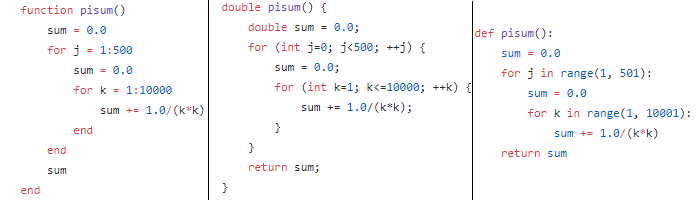
\includegraphics[scale=2.5]{bilder/pisum.png}
  \caption{Berechnung der Reihesumme $\sum_{q=0}^{10000} \frac{1}{q^{2}}$ 500 - mal in Julia, C und Python v. l. n. r. }
  \label{fig:pisum}
\end{figure}

\begin{figure}[hbt!]
  \centering
  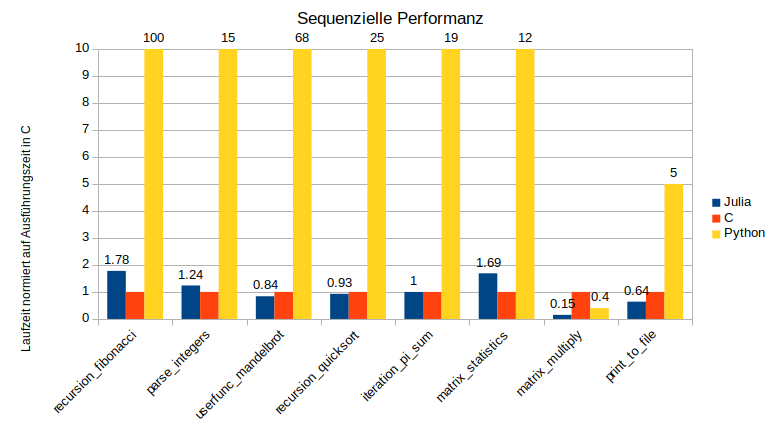
\includegraphics[scale=0.8]{bilder/sequenziell_performance.png}
  \caption{sequenzielle Performanz von Julia, C und Python für verschiedene Benchmarks}
  \label{fig:sequPerform}
\end{figure}

Wie in Abbildung~\ref{fig:sequPerform} zu sehen, ist hierbei Python teils deutlich langsamer und verlangte sogar eine Eingrenzung der Skale, da es bei \verb|recursion_fibonacci| \zB mehr als das 100-fache der Zeit, die C für den gleichen Algorithmus benötigt hatte, brauchte. So fällt neben diesem deutlich schlechterem Abschneiden von Python vorallem auf, das Julia etwa ähnlich schnell wie C,  bisweilen sogar schneller als C lief, was aber eindeutig den Benchmarks und dessen verminderter Aussagekraft an dieser Stelle zuzuschreiben ist. Allerdings erkennt man \zB auch an der Stelle für die Matrix-Matrix-Multiplikation, wie schnell Julias Code werden kann, wenn der Compiler in diesem Fall beispielweise zusätzliche Informationen über die Art der Matrizen erhält. Julia stellt damit vorallem unter Beweis, Python als Sprache für das Rapid-Prototyping ablösen zu können, da es eine ähnlichen angenehmen Syntax bietet, mit diesem aber eine viel bessere Laufzeit erreichen kann. Ein wichtiger Augenmerk sollte hier aber noch darauf gelegt werden, das Julia JIT compiliert. Dadurch kann der erste Aufruf einer Funktion wesentlich länger dauern, als folgende Aufrufe mit gleicher Argumentanzahl und Argumenttypen. (siehe Abbildung~\ref{fig:juliaPerform}) Nach diesem Erstdurchlauf geht die Geschwindigkeit aber aufgrund des zwischengespeicherten Machinencodes deutlich nach oben und ermöglicht Julia damit so viel schneller als Python zu sein.

\begin{figure}[hbt!]
  \centering
  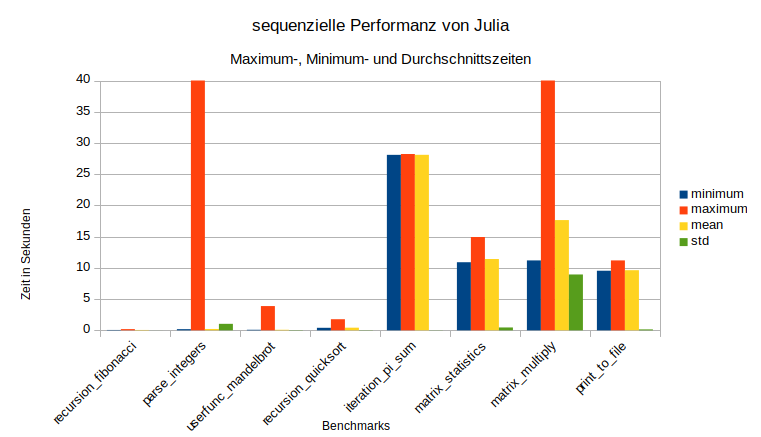
\includegraphics[scale=0.8]{bilder/julia_performance.png}
  \caption{Minimum-, Maximum-, Mean- und Standartwerte von Julia für die sequenzielle Performanz der verschiedenen Benchmarks }
  \label{fig:juliaPerform}
\end{figure}


%%%%%%%%%%%%%%%%%%%%%%%%%%%%%%%%%%%%%%%%%%%%%%%%%%%%%%%%%%%%%%%%%%%%%%%
\subsection{Laufzeittests für parallele Performanz in Julia}

Neben diesem Microbenchmarks wurden weiterhin Benchmarks für die oben aufgeführten parallelen Verfahren durchgeführt und gegen die sequenzielle Performanz gemittelt, um auch eine Aussagekraft über Julias Eignung auf einem HPC-System und den dort vorliegenden Anforderungen vorbringen zu können. Die Laufzeittests wurden mithilfe des Programms, veröffentlicht auf \cite{JuliaCookbook}, ermittelt. Betrachtet wurden hierbei die sequenzielle Performanz, die Performanz von \verb|@parallel|, das \verb|@parallel| Macro in Kombination mit der Reduktionsfunktion im speziellen die Addition \verb|(+)|, sowie \verb|pmap()| mit und ohne der Konfiguration von der Batchsiz  Größe. Die folgendene Abbildung~\ref{fig:CodeSnippet} zeigt ein Code-Snippet der genutzten Verfahren in ihrer Implementierung. Alle Verfahren wurden benutzt um die Summe über einem Array bzw einem SharedArray mit vorher festgelegter Länge zu berechnen. In den einzelnen Feldern des Arrays wurden vorher Werte durch eine Summenfunktion \verb|fun| über der Wurzel ausgerechnet und zurück geschrieben. Dabei werden die Laufzeittests in zwei Kategorien unterteilt: gute und mittlere Parallelisierbarkeit. Gute Parallelisierbarkeit bezeichnet hier wenige Funktionsaufrufe mit schwereren, aber weniger speicherverbrauchenden Funktionsberechnungen und mittlere Parallelisierbarkeit steht für mehr Funktionsaufrufe mit mittleren, mehr speicherverbrauchenden Funktionen. Dies wurde über die Parameter \verb|ProblemSize| und \verb|FunCalls| global konfiguriert, indem diese direkt den Aufwand für die Funktion \verb|fun| und die Größe der Arrays und damit auch der Funktionsaufrufe festlegten. Gut erkennbar ist zudem, wie ähnlich sich die einzelnen Implementierungen sehen. 

\begin{figure}[hbt!]
\begin{Verbatim}[baselinestretch=1,fontsize=\scriptsize,numbers=left,frame=single,stepnumber=5,xleftmargin=1cm,xrightmargin=1cm]
function simple_loop_sum(pt::Int,fun::Function=GlobalFun)
    a= Array{Float64}(FunCalls)
    for i=1:FunCalls; 
	a[i] = fun(ProblemSize); 
	end#for
    sum(a)
end#function##

function sharedarray_parallel_sum(pt::Int,fun::Function=GlobalFun)
    sa = SharedArray{Float64}(FunCalls)
    s= @sync @parallel for i=1:FunCalls; 
	sa[i] = fun(ProblemSize);
	 end#for
    sum(sa)
end#function

function sharedarray_mapreduce(pt::Int,fun::Function=GlobalFun)
    sa=SharedArray{Float64}(FunCalls)

    @parallel (+) for i=1:FunCalls; 
	sa[i]= fun(ProblemSize); 
	end#for
    sum(sa)
end#function

function pmap_sum_nb(pt::Int,fun::Function=GlobalFun)
    r = pmap( i-> fun(ProblemSize), 1:FunCalls )
    sum(r)
end#function

function pmap_sum_b(pt::Int,fun::Function=GlobalFun)
    r = pmap( i-> fun(ProblemSize), 1:FunCalls, 
	batch_size=ceil(Int,FunCalls/nworkers()))
    sum(r)
end#function
\end{Verbatim}
  \caption{Code-Snippets der benutzten Verfahren mit \textit{ProblemSize} als Problemgröße und  \textit{FunCalls} als Anzahl an Funktionsaufrufen}
 \label{fig:CodeSnippet}
\end{figure}

Abbildung~\ref{fig:taurusGood} zeigt die berechneten Werte für die verschiedenen Verfahren bei guter Parallelisierbarkeit in Abhängigkeit von der Anzahl der in Julia eingebundenen Prozessoren und dem Speedup, normiert an der sequenziellen Performanz. Gut zu erkennen ist, das sich für weniger, aber dafür größere Funktionsaufrufe die parallele Map gegen die For-Schleife durchsetzt und nochmals einen doppelten Speedup im vergleich zu dieser erzielen kann. Trotzdem ist auch die parallele For-Schleife um den Faktor fünf bis sechs schneller als die sequenzielle Performanz. Auffällig ist zudem das Sinken der Performanz beim Hinzufügen nur eines weiteren Prozessors, was sich durch die Implementierung des \textit{Master-Worker}-Prinzips in Julia erklären lässt. Da der erste Prozessor zum \textit{Master}-Prozessor wird, berechnet dieser nichts und die komplette Berechnung findet sequenziell auf dem Prozessor mit der Id zwei statt. Die Kosten für die Kommunikation und der Overhead, um den Prozess parallel zu machen, fallen aber trotzdem an, weshalb die Zeit, die der Algorithmus am Ende benötigt, sogar noch steigt. Das Festlegen der zu kopierenden Größe (Batchsize) für die parallele Map sorgt zudem für eine leicht bessere Performanz und verhindert, das die Kommunikation für ungünstige Situationen, wie etwa für zwei Prozessoren, den Algorithmus stark verlangsamt. Auch die Reduktionsfunktion der For-Schleife ist leicht schneller, was vorallem dem in diesen Messwerten nicht beachtetem Speichermanagment zuzuschreiben ist. Da die Reduktionsfunktion den Speicher effizienter verwaltet, kann sie schneller sein, belegt während der Ausführung vorallem aber auch weniger Speicher.

\begin{figure}
    \centering
    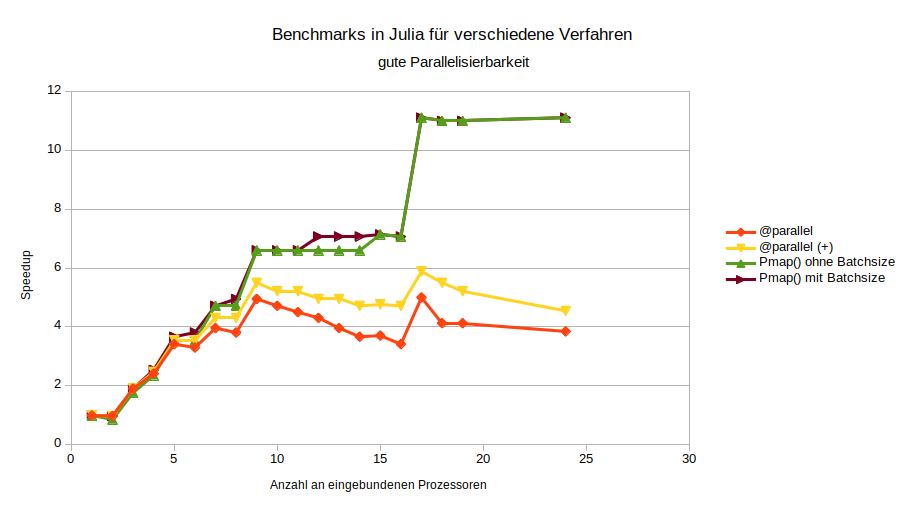
\includegraphics[scale=1, width=17cm]{bilder/parallel_performance_taurus_good.png} 
    \caption{Graph der Messwerte für gute Parallelisierbarkeit auf Taurus berechnet}
    \label{fig:taurusGood}
\end{figure}

Die Abbildung~\ref{fig:taurusMedium} zeigt die gemessenen Werte der einzelnen Verfahren bei mittlerer Parallelisierbarkeit wieder in Abhängigkeit der oben genannten Größen. Auffällig ist die sehr schlechte Performanz der \verb|Pmap() ohne Batchsize|. Mit bis zu 23-fachem Zeitaufwand verglichen mit der sequenziellen Performanz ist dieses Verfahren ohne das Spezifizieren der Batchsize nicht mehr lukrativ und verschlimmert sogar die Performanz des Algorithmus deutlich. Deshalb wird dieses Verfahren im weiteren nur noch mit einer festgelegten Batchsize betrachtet. Aber auch so ist die parallele Map nur noch um den Faktor zwei schneller als die sequenzielle Performanz und verliert damit deutlich auf die parallele For-Schleife im Vergleich zur Abbildung~\ref{fig:taurusGood}. Gut zu erkennen ist hierbei, das jedes Verfahren für seine Probleme optimiert ist und \verb|Pmap()| eher für größere Funktionen und \verb|@parallel| eher für viele kleinere Funktionen geeignet ist. Die parallele For-Schleife wird für mittlere Parallelisierbarkeit teilweise sogar noch schneller als für gute Parallelisierbarkeit und erreicht wieder einen Speedup ca um den Faktor fünf bis sechs. Auffällig ist auch, dass der Algorithmus sich nicht bis in das Unendliche beschleunigen lässt, durch das Hinzufügen von weiteren Prozessoren, sondern ab 14 eingebundenen Prozessoren durch Kontextwechsel und weiteren Kommunikationsaufwand anfängt, wieder etwas langsamer zu werden. Auch der bereits beobachtete Abfall der Performanz für zwei eingebundene Prozessoren lässt sich hier wieder beobachten und mit der gleichen Argumentation wie oben erklären.

\begin{figure}
    \centering
    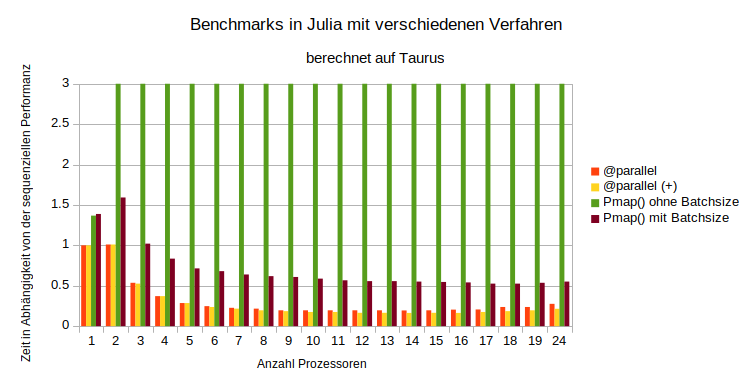
\includegraphics[scale=0.8, width=17cm]{bilder/parallel_performance_taurus_medium}
    \caption{Graphen der Messwerte für mittlere Parallelisierbarkeit auf Taurus berechnet}
    \label{fig:taurusMedium}
\end{figure}
\newpage
%%%%%%%%%%%%%%%%%%%%%%%%%%%%%%%%%%%%%%%%%%%%%%%%%%%%%%%%%%%%%%%%%%%%%%%
\section{Zusammenfassung}

In dieser wissenschaftlichen Ausarbeitung wurden Julia hinsichtlich der Kriterien Handhabbarkeit und Performanz für High-Performanz-Programmierung analysiert. Dazu wurden im ersten Teil Julias Schlüsselfunktionen betrachtet und darauf untersucht, wie sich Julia deren Vorteile Zunutze macht und gleichzeitg deren Schwachstellen ausgleicht etwa durch das Speichern von Maschinencode. Im zweiten Teil wurde  dann Bezug zur High-Performanz-Programmierung hergestellt, indem sich ausführlich mit Möglichkeiten zur Parallelisierung und Geschwindigkeitserhöhung auch unter Betrachtung von Fallstricken in Julia beschäftigt wurde. Dabei wurde zuerst über Funktionen im Hintergrund von Julia gesprochen, die die Parallelität gewährleisten. Im Anschluss wurden die gängisten Verfahren zur parallelen Programmierung mit Julia vorgestellt und zum Schluss noch etwas über weiterführende Themen und hilfreiche Werkzeuge gesagt. Im dritten und abschließenden Teil wurden dann die Eignung von Julia als High-Performanz-Sprache untersucht. Hierfür wurden sequenzielle Tests gegen C und Python durchgeführt und ausgewertet und anschließend noch oben angesprochenen Verfahren hinsichtlich ihrer Performanz für unterschiedlich gut zu parallelisierenden Fällen betrachtet. 
Julia kann eine sehr praktische und auch schnelle Sprache sein. Viele der getesteten Algorithmen konnte Julia teils deutlich beschleunigen ohne dabei den angenehmen Syntax von Python aufgeben zu müssen. Die Kombination aus typoptimierten Code mit einem Compiler, dem man Details mitgeben kann, wie etwa die innere Struktur einer Matrix, sorgt für sehr gute sequenzielle Geschwindigkeiten, sofern die Funktionen vorher bereits einmal ausgeführt worden waren und fast ausschließlich gespeicherter Maschinencode benutzt werden kann. Auch für High-Performanz-Programmierung bietet Julia viele angenehme Funktionen, die Algorithmen in ihrer Ausführung stark beschleunigen, sofern man einige Fallstricke beachtet und weiß, wie man dieses Problem am besten optimiert. Julia kann, wie im Projekt Celeste~\cite{CelesteNextPlatform} beschrieben, einen sehr großen Speedup erreichen und sich sogar fast mit der Geschwindigkeit von C messen lassen und kann damit zurecht behaupten, Python als Rapid-Prototyping-Sprache zu verdrängen und durch kleine Optimierungen und Analysen des Julia-Codes mit Werkzeugen auf die Auslagerung in C Routinen verzichten zu können. 
Auch bestehende Bibliotheken aus anderen Sprachen lassen sich sehr einfach einbinden und ausführen und erreichen dabei zumeist noch ähnliche Geschwindigkeiten, wie in der ursprünglichen Sprache. Auch die Communty ist sehr aktiv und hilfsbereit, wodurch sich der Einstieg in diese noch sehr junge Sprache deutlich vereinfachen lässt. Ein großer Nachteil den Julia allerdings immer noch mit sich bringt und der dafür sorgt, das sich die Sprache bisher noch nicht etablieren konnte, ist dessen Instabilität und häufigen Patches aufgrund der Beta-Version in der sie sich aktuell noch befindet. Selbst eigentlich aktuelle Pakete, wie die Microbenchmarks, erfordern Anpassungen im Quellcode um ausgeführt werden zu können. Mit im Zusammenhang dazu steht auch die Softwareumgebung \ua die vielen Pakete und Tools, die es bereits gibt, die aber wie \zB der Debugger teilweise einfach noch nicht mit der aktuellen Version im vollem Umfang funktionieren und dadurch gerade die Entwicklung von Anwendungen, die nicht auf numerisches Rechnen ausgelegt sind, erschweren und notwendig machen, sich selbst mit den Paketen und deren Implementierung zu befassen. Dadurch fühlt sich Julia bisweilen auch noch etwas mühselig an. Trotz alledem ist Julia eine interessante neue Sprache, die es durch aus Wert ist, weiter untersucht zu werden. Gerade nach dem ersten öffentlichen Release sollte sie als Konkurrent zu Python und C betrachtet werden und als Programmiersprache für ein Projekt zumindest überdacht werden.
\end{document}
